\documentclass{article}
\usepackage[utf8]{inputenc}
\usepackage{listings}
\usepackage{xcolor}
\usepackage{amsmath}
\usepackage{subfiles}
\usepackage{hyperref}
\usepackage{graphicx}
\usepackage{float}
\usepackage[a4paper, total={6.5in, 8in}]{geometry}
\setlength{\topmargin}{-1cm}
\hypersetup{
    colorlinks=true,
    linkcolor=red,
    filecolor=magenta,      
    urlcolor=cyan,
}

\definecolor{codegreen}{rgb}{0,0.6,0}
\definecolor{codegray}{rgb}{0.5,0.5,0.5}
\definecolor{codepurple}{rgb}{0.58,0,0.82}
\definecolor{backcolour}{rgb}{0.95,0.95,0.92}
\lstdefinestyle{mystyle}{
    backgroundcolor=\color{backcolour},   
    commentstyle=\color{codegreen},
    keywordstyle=\color{magenta},
    numberstyle=\tiny\color{codegray},
    stringstyle=\color{codepurple},
    basicstyle=\ttfamily\footnotesize,
    breakatwhitespace=false,         
    breaklines=true,                 
    captionpos=b,                    
    keepspaces=true,                 
    numbers=left,                    
    numbersep=5pt,                  
    showspaces=false,                
    showstringspaces=false,
    showtabs=false,                  
    tabsize=2
}

\lstset{style=mystyle}
\definecolor{MycolorOrange}{HTML}{ff821a}


\title{AOOP Assignment 1 }
\author{elias.vahlberg.2 }
\date{April 2021}

\begin{document}

\maketitle
    %\hypertarget{E1}{ }


\section*{Overview}
Document links:
\begin{itemize}
\item \hyperlink{E1}{Exercise 1}
\item \hyperlink{E2}{Exercise 2}
\item \hyperlink{E3}{Exercise 3}
\item \hyperlink{E5}{Exercise 5}
\item \hyperlink{E6}{Exercise 6}
\item \hyperlink{E7}{Exercise 7}
\item \hyperlink{E8}{Exercise 8}
\item \hyperlink{E9}{Exercise 9}
\item \hyperlink{E10}{Exercise 10}
\item \hyperlink{E12}{Exercise 12}
\item \hyperlink{E13}{Exercise 13}
\item \hyperlink{E14}{Exercise 14}
\item \hyperlink{E15}{Exercise 15}
\end{itemize}

\section*{Exercises}

\subsection*{1) (*) Exercise 2.9 in the course book.}
\hypertarget{E1}{ }
\textit{What relationship is appropriate between the following classes: aggregation,
inheritance, or neither?}\\
\indent \textbf{\textcolor{blue}{Solution:}} \\
\textbf{a) Student–Course}\\
\indent (n,n) \\
\indent    One student can have multiple courses.\\
\indent    One course can have multiple students.\\
\textbf{(b) Course–Section}\\
\indent    (1,n)\\
\indent    One section can only belong to one course.\\
\indent    One course can have multiple sections.\\
\textbf{(c) Section–Instructor}\\
\indent    (n,n)\\
\indent    One section can have multiple instructors.\\
\indent    One instructor can have multiple sections.\\
\textbf{(d) Section–Room}\\
\indent    (n,n)\\
\indent    One section can use multiple rooms.\\
\indent    One room can be used by multiple sections.\\



\subsection*{2) Exercise 2.12 in the course book.}
\hypertarget{E2}{ }
\textit{Consider an online store that enables customers to order items from a catalog and
pay for them with a credit card. Draw a UML diagram that shows the relationships
between these classes:}\\
\indent \textbf{\textcolor{blue}{Solution:}} \\
\begin{figure}[H]
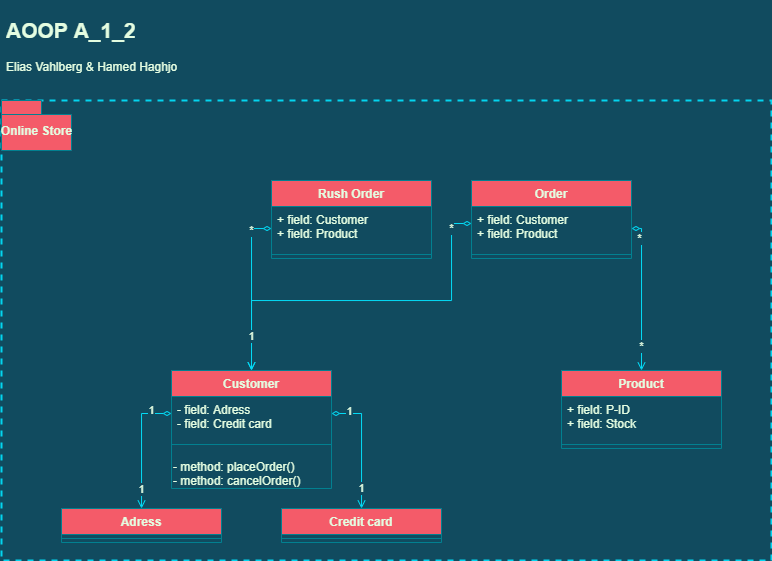
\includegraphics[width=\linewidth]{AOOP_A1_2}
\centering
\end{figure}
\newpage


\subsection*{3) Exercise 2.13 in the course book.}
\hypertarget{E3}{ }
\textit{Consider this test program:}
\lstinputlisting[language=Java]{Tester.java}
\textit{Draw a sequence diagram that shows the method calls of the main method.} \\
\indent \textbf{\textcolor{blue}{Solution:}} \\
\begin{figure}[H]
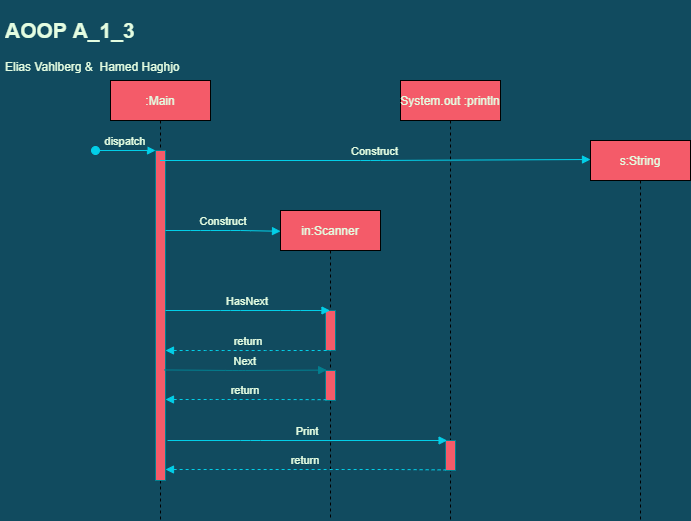
\includegraphics[width=\linewidth]{AOOP_A1_3}
\centering
\end{figure}


\subsection*{5) (*) Exercise 3.8 in the course book}
\hypertarget{E5}{ }
\textit{Implement a class Matrix that represents a matrix}\\
$$ 
M = \left( 
\begin{matrix}
a_{0,0} & a_{0,1} & \cdots & a_{0,c-1} \\
a_{1,0} & a_{1,1} & \cdots & a_{1,c-1} \\
\vdots & \vdots & \ddots & \vdots \\
a_{r-1,0} & a_{r-1,1} & \cdots & a_{r-1,c-1} 
\end{matrix} \right)
$$
\textit{
where r and c are the number of rows and columns of the matrix. Your class should support the
following operations:}\\
\begin{itemize}
    \item Constructs a matrix with a given number of rows and columns.
    \item Gets and sets the element at a particular row and column position.
    \item Adds and multiplies two compatible matrices.
\end{itemize}
\indent \textbf{\textcolor{blue}{Solution:}} \\
\hyperlink{Matrix}{Matrix.java}

\subsection*{6) (*) List three immutable classes from the standard library.}
\hypertarget{E6}{ }
\indent \textbf{\textcolor{blue}{Solution:}} \\
\textcolor{MycolorOrange}{Java.util.UUID} \\
\textcolor{MycolorOrange}{Java.util.Locale} \\
\textcolor{MycolorOrange}{java.lang.StackTraceElement}


\subsection*{7) (*) Implement and test a stack data type.}
\hypertarget{E7}{ }
\begin{itemize}
    \item Implement the stack data type with integer elements.
    \item Implement the functions push and pop.
    \item Implement a push function that inserts a set of \textit{n} elements.
    \item Implement a pop function that returns a set of \textit{n} elements.
\end{itemize}
\indent \textbf{\textcolor{blue}{Solution:}} \\
\hyperlink{IntStack}{IntStack.java}\\
\hyperlink{IntStackTest}{IntStackTest.java}

\subsection*{8) (*) Exercises 3.20 and 3.21 in the course book.}
\hypertarget{E8}{ }
\textit{Improve the circular array implementation of the
bounded queue by growing the elements array when the queue is full. Add assertions to check
all preconditions of the methods of the bounded queue implementation.}\\
\indent \textbf{\textcolor{blue}{Solution:}} \\
\hyperlink{MessageQueue}{MessageQueue.java}\\
\hyperlink{MessageQueueTest}{MessageQueueTest.java}

\subfile{section9.tex}
\newpage
\subfile{AppendixCode.tex}

\end{document}
